\documentclass[a4paper, 10pt]{article}
\usepackage[utf8x]{inputenc}
\usepackage{graphicx}
\usepackage{mathenv}
\usepackage{geometry}
\geometry{hmargin = 2.5cm, vmargin = 1.5cm}

% OPENING
\title{SY19 - TP03\\Réseaux de Neurones : Optimisation de l'Architecture}
\author{Alice Ngwembou - Antoine Hars}

\begin{document}

\maketitle

\section*{Introduction}
Le but de ce TP est la mise en oeuvre d'un algorithme basé sur les réseaux de neurones pour la classification.

\section*{Exercice 1}

\section*{Exercice 2}

\subsection*{Travail Préliminaire}

\subsubsection*{Question 1 :}

\textbf{1. Quelles sont les 4 lois utilisées pour générer les observations de l’ensemble d’apprentissage appartenant à 4 places ?}\\
Nous avons 4 lois Normales $\mathcal{N}(\mu_{1}, \Sigma_{1})$, $\mathcal{N}(\mu_{2}, \Sigma_{2})$, $\mathcal{N}(\mu_{3}, \Sigma_{3})$ et $\mathcal{N}(\mu_{4}, \Sigma_{4})$ avec :\\ \\
\hspace*{0.5cm}
\begin{tabular}{cccc}
$\mu_{1}$ = (4, 6) &
$\Sigma_{1}$ = $\begin{pmatrix} 1 & 0 \\ 0 & 2 \end{pmatrix}$ &
$\mu_{2}$ = (6, 1) &
$\Sigma_{2}$ = $\begin{pmatrix} 2 & 0 \\ 0 & 1 \end{pmatrix}$\\ \\
$\mu_{3}$ = (-4, 4) &
$\Sigma_{3}$ = $\begin{pmatrix} 1.5 & 0 \\ 0 & 2 \end{pmatrix}$ &
$\mu_{4}$ = (0, 0) &
$\Sigma_{4}$ = $\begin{pmatrix} 1 & 0 \\ 0 & 1 \end{pmatrix}$\\
\end{tabular}\\ \\ \\
\textbf{2. Donner la règle de Bayes qui permet de répondre à un problème de classification à c classes.}\\
%TODO
\textbf{3. Développer la règle de Bayes pour arriver à la solution donnée dans le code ci-dessus.}\\
%TODO

\subsection*{Réseaux de neurones sur des données simulées}

\subsubsection*{Question 2 :}

\textbf{1. Dessiner le frontières de décision obtenues avec un réseau de neurones sur les données (pour decay = 0 et size = 5.)}\\
L'exécution du code donnée nous permet d'observer le graphique suivant :\\
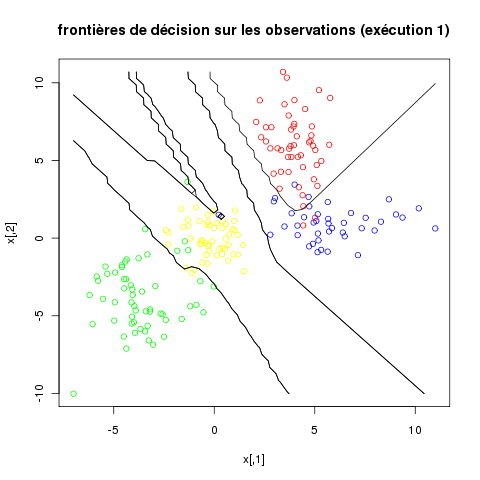
\includegraphics[height = 7cm, width = 7cm]{plots/frontiere_bayes_q2_1.png}\\
Nous pouvons observer sur ce graphiques les différentes observations de l'ensemble d'apprentissage avec une couleur précise et les frontières de décision obtenues.\\
On peut dire que tous les points de chaque loi normale ne se situent pas exactement du bon coté des frontières de décision.\\ \\
\textbf{2. Visualiser l'estimation des poids.}\\
%TODO
\textbf{3. Obtient-on les mêmes résultats à chaque fois pour l'estimation des poids et des frontières de décision lorsqu'on lance plusieurs fois la procédure $nnet$ ?}\\
En relançant la procédure $nnet$, nous n'obtenons pas les mêmes frontières de décision.\\
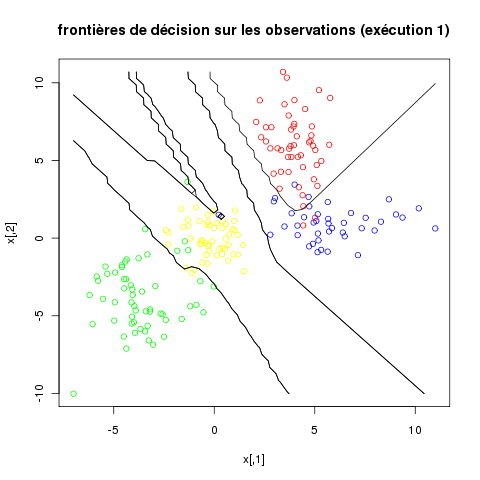
\includegraphics[height = 7cm, width = 7cm]{plots/frontiere_bayes_q2_1.png}
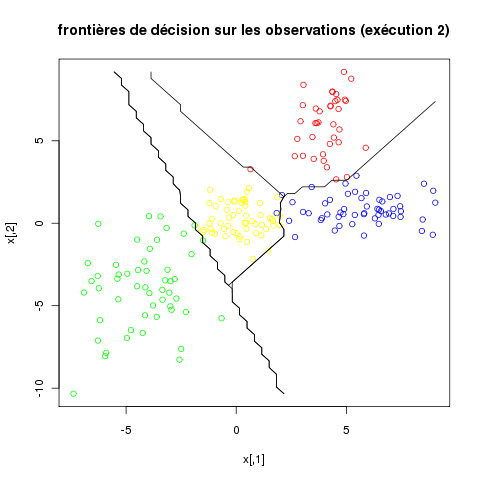
\includegraphics[height = 7cm, width = 7cm]{plots/frontiere_bayes_q2_2.png}\\
\textbf{4. Comment expliquer ce phénomène ?}\\
%TODO
il semble que ce phénomène vient du fait que le générateur de nombre aléatoire de R n'est pas réinitialisé entre les 2 exécutions de $nnet$.

\subsubsection*{Question 3 :}

On désire voir l'influence du nombre de neurones dans la couche cachée. Pour cela, pour decay = 0, faire varier size de 1 à 10 (nombre de neurones dans la couche cachée).\\ \\
\textbf{1. Commenter le nombre de "poids" à estimer.}\\
%TODO
\textbf{2. Afficher les frontières de décision (4 seulement). Que constater sur la forme des frontières et sur le nombre de points mal-classés quand size augmente ?}\\
%TODO
\textbf{3. Relancer la procédure sur un nouveau jeu de données en faisant varier size de 1 à 10.}\\
%TODO
\textbf{4. Que dire de la variabilité du modèle en fonction de size ?}\\
%TODO

\subsubsection*{Question 4 :}

On désire voir l'influence du paramètre de régularisation.\\ \\

\textbf{1. Pour size = 5, comparer l'estimation des poids et des frontières pour decay = 0.001, 0.01, 0.1, 1, 10, 100.}\\
%TODO
\textbf{2. Que dire de la valeur des poids optimaux quand decay augmente ?}\\
%TODO
\textbf{3. Comment expliquer ce phénomène et comment cela se traduit-il sur la forme des frontières ?}\\
%TODO

\subsection*{Classification des données Crabes}

\subsubsection*{Question 5 :}

\subsubsection*{Question 6 :}

\section*{Conclusion}

\end{document}
